\chapter{\label{ch:5-Loop equations for Boundary Conditions in the 3-state Potts Model} Boundary Conditions in the 3-state Potts Model}

%The free variable approach to loop equations is a simple but powerful method for computing correlation functions in matrix models. In the case of the one-matrix model the set of loop equations is exhausted by considering the infinitesimal variation of the underlying degrees of freedom by the resolvent operator. This is sufficient to determine the spectral curve for the one-loop function and compute the continuum limit. For the two-matrix model with an action that is a polynomial in the two matrix degrees of freedom, considering the corresponding loop equation is not sufficient to determine the one-loop function. By a number of appropriately selected variations one may construct the spectral curve of the one-loop function in the simplest situation where there is a single quadratic interaction term coupling the two matrices. However this is not sufficient to compute the spectral curve for generic two-matrix models or higher order multi-matrix models.

%In this chapter we consider the construction of the planar disk amplitude of the 3-state Potts model for various boundary conditions using the loop equation method. The loop equation method is in one-to-one correspondence with the combinatorial description of expressing the removal of a given boundary edge in terms of the number possible graphs that can be obtained and so this problem is equivalent to the combinatorial problem of counting the number of planar random graphs with specified boundary configurations. This problem was previously addressed using the saddle-point approach in \cite{Niedner:2016skw}, and so another aim of this chapter is to confirm these results using an independent method.

%This chapter is structured as follows: first we describe the general loop equation method we employ for calculating planar resolvents, which contrasts with the loop equation method of Eynard \cite{Eynard:2002kg, Eynard:1999gp}, and we use the two-matrix model with a generic cubic potential as an example model to demonstrate its strengths. Following this we compute the resolvents corresponding to fixed, mixed, and free boundary conditions for the 3-state Potts matrix model. In the case of the mixed boundary condition the structure of the resolvent is more complex, and we discuss how it is consistent with the results of \cite{Niedner:2016skw} using the saddle-point approach. Finally we determine the free boundary condition, and discuss the limits of the method by attempting to calculate the $U$-boundary condition of chapter 4. In this chapter we omit the final result for the spectral curves and list these large expressions in appendix B.

Since the work of Eynard and Bonnet \cite{Eynard:1999gp}, it has been known that the planar
resolvent, corresponding to the fixed spin boundary conditions of the 3-state Potts model on random
planar graphs, may be computed through the method of loop equations. The work of Atkin, Niedner and
Wheater \cite{Niedner:2016skw}, building on the saddle-point approach of Daul \cite{Daul:1994qy},
and subsequently Zinn-Justin \cite{ZinnJustin:1999jg}, demonstrated that the saddle-point method
may be used to compute the planar eigenvalue density distribution for the sum of $p$ random
matrices in the $q$-state Potts model, and thus a wider variety of boundary conditions. As
discussed in Chapter 2, the method of loop equations has a direct combinatorial interpretation,
expressing the possible ways of decomposing random graphs after the removal of a marked edge.
Whether one could recover the results of \cite{Niedner:2016skw} in this language is the the
question we seek to address in this chapter.

This chapter is organised as follows. In Section 5.1 we describe the formalism we use to discuss
loop equations for general multi-matrix models, which we subsequently demonstrate for the
particular case of the two-matrix model with a generic cubic potential. In Section 5.2 we then
describe an algorithm for computing and systematically solving loop equations. We immediately apply
this to the case of the 3-state Potts model in Section 5.3, where we illustrate the algorithm in
detail for the $p=1$ fixed spin resolvent. We then discuss the case of the $p=2$ mixed and $p=3$
free boundary conditions, and describe general features of the spectral curve. Further to this, we
discuss some non-standard boundary conditions, which includes a case where the loop equation method
fails. Finally, in Section 5.4 we consider the case of the dilute Ising model, followed by the
dilute 3-state Potts model in Section 5.5, before concluding with a discussion of some implications
of our results.

\section{Formalism}

Consider a generic multi-matrix model in $n$ Hermitian matrix degrees of freedom
$\mathbf{X}=\{X_i\}_{i=1}^n$ of the form
%
\begin{equation}
    \label{loops1}
    Z = \int \prod_{i=1}^n [dX_i] \, e^{-N\text{Tr}V(\mathbf{X})},
\end{equation}
%
where $V(\mathbf{X})$ is a potential function which is a polynomial of degree $d+1$ in the $n$
matrices of $\mathbf{X}$, and depends on couplings $\{t_i\}_{i=2}^{\infty}$. We are interested in
computing the planar resolvent of a given matrix, say $X \coloneqq X_1$.

Define the following resolvent functions with boundary insertions
%
\begin{equation}
    \label{loopRes}
    W_{w(\mathbf{X})}(z) = \frac{1}{N} \left\langle \text{Tr} \frac{1}{2} \big( w(\mathbf{X}) + \bar{w}(\mathbf{X})\big) \frac{1}{z-X} \right\rangle,
\end{equation}
%
where $w(\mathbf{X})$ is a word in the free algebra generated by $\mathbf{X}$ and
$\bar{w}(\mathbf{X})$ the reversed word, but with the constraint that $X$ is not the first or last
letter of the word. On the left hand side we will proceed to label the resolvent functions by the
indices labelling the matrices that comprise the word $w(\mathbf{X})$ for the sake of brevity.
Hence, one may write
%
\begin{equation}
    \label{resExample}
    W_{(2,1,3)}(z) = \frac{1}{N} \left\langle \text{Tr} \frac{1}{2} (X_2 X_1 X_3 + X_3 X_1 X_2 ) \frac{1}{z-X} \right\rangle.
\end{equation}
%
Furthermore, we define the following trace correlation functions analogously,
%
\begin{equation}
    \label{trace}
    p_{w(\mathbf{X})}= \frac{1}{N} \left\langle \text{Tr} \frac{1}{2} (w(\mathbf{X}) + \bar{w}(\mathbf{X}))\right\rangle.
\end{equation}
%
Define the level of a resolvent function of the form \eqref{loopRes} as the length of the
associated word, $L(w(\mathbf{X}))$, such that, for example, \eqref{resExample} with $L(X_2 X_1
    X_3)=3$ denotes a level-3 resolvent function. Similarly, we index trace correlation functions of a
given level by the set of words of appropriate length.

The number of inequivalent trace correlation functions of a given level is generally much smaller
than the size of the corresponding set of words. Due to cyclicity of the trace and symmetry under
reversal of the word (which has been arranged by construction in \eqref{trace}), there is a $D_k$
symmetry for the correlators, where $D_k$ is the dihedral group of order $k$. There may also be a
global symmetry, $G$, of the matrix model potential, given by
%
\begin{equation}
    \label{symmetry}
    G = \{ g\in \text{Aut}(\mathbf{X}) : V(g(\mathbf{X}))=V(\mathbf{X})\}.
\end{equation}
%
An example of this would be permutation symmetry amongst the matrix degrees of freedom. Therefore,
defining the set of irreducible trace correlation functions of level $k$ as $\mathcal{P}_k$, we may
write
%
\begin{equation}
    \label{irreducibleTrace}
    \mathcal{P}_k \cong \mathbf{X}^k / (D_k \times G).
\end{equation}
%
The number of inequivalent correlators is then given by the cardinality of this set.

Similarly we define the set of irreducible resolvent functions of level $k$ as $\mathcal{W}_k$. The
number of independent resolvent functions is also constrained, although not as severely as the
correlation functions are. Define the operator $\Delta$, acting on resolvent functions as follows:
%
\begin{align}
    \label{delta}
    \Delta^k W_{w(\mathbf{X})}(z) & : = \frac{1}{N} \left\langle \text{Tr}\frac{1}{2} \big( X^k w(\mathbf{X}) + \bar{w}(\mathbf{X})X^k\big) \frac{1}{z-X}\right\rangle \\
                                  & = z^k W_{w(\mathbf{X})}(z) - \sum_{i=1}^k z^{k-i} p_{X^{k-1}w(\mathbf{X})}.
\end{align}
%
We may omit words for which any sub-word consisting only of the matrix $X$ adjoins the loop
operator $(z-X)^{-1}$, since these may be expressed in terms of the $\Delta$ operator to a power
given by the length of the adjoining sub-word in $X$, acting on a lower-level resolvent function.
Moreover, the presence of the loop operator means that, relative to the correlation functions, the
dihedral symmetry is reduced as $D_k\rightarrow\mathbb{Z}_2$, corresponding to symmetry under
reversal of the words defining the resolvent functions. Finally, having fixed $X$ as the
representative matrix of the loop operator, the defining word only respects the subgroup
$G'\subseteq G$, consisting of elements $g\in\text{Aut}(\tilde{\mathbf{X}})$, where
$\tilde{\mathbf{X}}=\mathbf{X} \setminus X$. Therefore we may write
%
\begin{equation}
    \label{irreducibleResolvent}
    \mathcal{W}_k \cong (\tilde{\mathbf{X}} \times \mathbf{X}^{k-2} \times \tilde{\mathbf{X}})/(\mathbb{Z}_2 \times G').
\end{equation}

For example, consider a three-matrix model with matrix degrees of freedom $X_1,X_2,X_3$, with a
$\mathbb{Z}_2$ symmetry under exchange of $X_1$ and $X_2$. Then for the resolvent functions with
respect to $X_1$, one would find $ W_{(3,2,1,2,3)} \neq W_{(3,1,2,1,3)}$, and therefore the
representative words comprise two distinct elements of $\mathcal{W}_5$, whereas the same words are
identified in $\mathcal{P}_5$ as one has $p_{3,2,1,2,3} = p_{3,1,2,1,3}$.

Loop equations are Schwinger-Dyson equations of the matrix model, expressing the invariance of the
matrix integral under infinitesimal reparameterisations $X_i \rightarrow X_i + \varepsilon \delta
    X_i$. There is some freedom as to which variations one can consider. In Chapter 2 we outlined one
approach, specific to the two-matrix model, where one studies reparameterisations using products of
the resolvent operator \eqref{var2}. The approach we adopt here is to consider variations of the
form
%
\begin{equation}
    \label{reparam}
    \delta X_i = w_1(\mathbf{X}) \frac{1}{z-X} w_2(\mathbf{X}) + \bar{w}_2(\mathbf{X})\frac{1}{z-X}\bar{w}_1(\mathbf{X}).
\end{equation}
%
One then evaluates the loop equation by equating the first order contribution from the Jacobian,
which may be computed using the split rule \eqref{Jsplit}, with the contribution from the potential
\eqref{loop}. These reparameterisations are manifestly Hermitian, and the resulting constraints may
be expressed in terms of the resolvent functions \eqref{loopRes} and trace correlation functions
\eqref{trace}.

We can classify loop equations by the level of their highest-level resolvent functions. If
$V'(\mathbf{X})$ is degree $d$ in $\tilde{\mathbf{X}}$\footnote{The degree will generally be
    different for variations corresponding to different $X_i\in\mathbf{X}$.}, then level-$k$ loop
equations are given by \eqref{reparam} with $L(w_2)=k-d-L(w_1)$. We can therefore define a
corresponding set of level $k$ variations,
%
\begin{equation}
    \label{var}
    \mathcal{V}_k = \left\{ (w_1,w_2)\in\mathbf{V}_m\times\overline{\mathbf{V}}_{k-d-m} : m=k-d,\cdots \ceil{(k-d)/2} \right\},
\end{equation}
%
where $\mathbf{V}_m=\mathbf{X}^{m-1}\times \tilde{\mathbf{X}}$ and $\overline{\mathbf{V}}_m =
    \tilde{\mathbf{X}}\times\mathbf{X}^{m-1}$. That is, the words $w_1$ and $w_2$ are constrained such
that the letters in contact with the loop operator are in $\tilde{\mathbf{X}}$. This is so that the
resulting loop equations are distinct from lower-level loop equations.

The key idea of the loop equation approach we adopt is to compute the Schwinger-Dyson constraints
for each matrix degree of freedom by a sufficiently large set of variations. We aim to compute loop
equations up to a certain level $n_{\text{max}}$, which denotes the level at which the number of
algebraically independent constraints outnumber the total number of independent resolvent functions
present in the constraints, and then eliminate the resolvent functions so that we obtain an
algebraic equation for the planar (level-0) resolvent. This may be regarded as a discrete version
of the approach outlined in Chapter 2, since one may expand the product of resolvent operators as
an infinite sum of words in matrices of arbitrary length multiplying a single resolvent operator.
It is hoped that this refined set of equations contains more information than if one only considers
a finite set of reparameterisations by products of loop operators, allowing us to compute the
planar resolvent.

\subsection{The two-matrix model with generic cubic potential}

To illustrate our formalism and demonstrate the strength of the loop equation approach, let us
consider the simple example of a two-matrix model with a generic cubic potential:
%
\begin{align}
    \label{2MMGeneric}
    V(M_1,M_2) = & \frac{1}{2(\alpha \beta - \gamma^2)}(\alpha M_1^2 + \beta M_2^2 - 2 \gamma M_1 M_2) \\
                 & \qquad \quad \nonumber + \frac{1}{3} (a M_1^3 + 3b M_1^2 M_2 + 3d M_1 M_2^2 + e M_2^3).
\end{align}
%
This furnishes an example of a multi-matrix model which is not solvable through any known
saddle-point or orthogonal polynomial approach. In particular, the loop equation method of Chapter
2 is not sufficient to compute the planar resolvent. However, as first demonstrated in
\cite{Carroll:1995nj}, one may compute the resolvent of this model using our more granular loop
equation strategy.

For \eqref{2MMGeneric} the following are the minimal set of reparameterisations:
%
\begin{align}
    \label{2MMGenericReps}
    \delta M_{i} & = \frac{1}{z-M_1}, \\
    \delta M_{i} & = M_2 \frac{1}{z-M_1} + \text{h.c.}, \\
    \delta M_{i} & = M_2^2 \frac{1}{z-M_1}+\text{h.c.}, \\
    \delta M_{i} & = M_2 \frac{1}{z-M_1} M_2,
\end{align}
%
for $i\in\{1,2\}$. Calculating the corresponding loop equations yields the following relations,
where the action of the $\Delta$ operator is given by \eqref{delta} for $k=1$, i.e.
$\Delta^1=\Delta$, and we suppress the $z$-dependence of the resolvent functions\footnote{Note that
    $W_2$ is distinct from the resolvent $W_{(2)}$ \eqref{eq2}, which denotes the resolvent of the sum
    of two matrices.}:
%
\begin{align}
    W^2 =             & -d W_{(2,2)}+\frac{\gamma  W_{2}}{\gamma ^2-\alpha  \beta }-a\Delta^2 W -2b \Delta W_{2} +\frac{\alpha \Delta W}{\alpha  \beta -\gamma ^2}, \\
    0 =               & -e W _{(2,2)}+\frac{\beta  W_{2}}{\alpha  \beta -\gamma ^2} - b\Delta^2 W  - 2d\Delta W_{2}+\frac{\gamma \Delta W}{\gamma ^2-\alpha  \beta }, \\
    W  W_{2} =        & \frac{\gamma  W_{(2,2)}}{\gamma ^2-\alpha  \beta }-a\Delta^2 W_{2} -b \Delta W_{(2,2)} -b W_{(2,1,2)}-d W_{(2,2,2)}+\frac{\alpha  \Delta W_{2}}{\alpha  \beta -\gamma ^2}, \\
    W =               & \frac{\beta  W_{(2,2)}}{\alpha  \beta -\gamma ^2}-b \Delta^2 W_{2}-d\Delta W_{(2,2)}-d W_{(2,1,2)}-e W_{(2,2,2)}+\frac{\gamma \Delta W_{2}}{\gamma ^2-\alpha  \beta }, \\
    W  W_{(2,2)} =    & \frac{\gamma  W_{(2,2,2)}}{\gamma ^2-\alpha  \beta }-a\Delta^2 W_{(2,2)}-b\Delta W_{(2,2,2)}-b W_{(2,1,2,2)}-d W_{(2,2,2,2)}+\frac{\alpha  \Delta W_{(2,2}}{\alpha  \beta -\gamma ^2}, \\
    W  p_{2}+ W_{2} = & \frac{\beta  W_{(2,2,2)}}{\alpha  \beta -\gamma ^2}-b\Delta^2 W_{(2,2)}-d\Delta W_{(2,2)}-d W_{(2,1,2,2)} -e W_{(2,2,2,2)}+\frac{\gamma \Delta W_{(2,2)}}{\gamma ^2-\alpha  \beta }, \\
    W_{2}^2 =         & \frac{\alpha  W_{(2,1,2)}}{\alpha  \beta -\gamma ^2}+\frac{\gamma  W_{(2,2,2)}}{\gamma ^2-\alpha  \beta }-a W_{(2,1,1,2)}-2 b W_{(2,1,2,2)}-d W _{(2,2,2,2)}, \\
    2 W_{2} =         & \frac{\gamma  W_{(2,1,2)}}{\gamma ^2-\alpha  \beta }+\frac{\beta  W_{(2,2,2)}}{\alpha  \beta -\gamma ^2}-b W_{(2,1,1,2)}-2 d W_{(2,1,2,2)}-e W_{(2,2,2,2)}.
\end{align}
%
These are eight independent equations in eight unknowns which may be eliminated to give a single
algebraic equation for the resolvent $W(z)$. This spectral curve is degree 4 in both the resolvent
and the boundary cosmological constant. We can, at most, tune the parameters of the model to
achieve critical behaviour of the form $W(z)\sim(z-z_c)^{4/3}$, which is characteristic of the
critical Ising model universality class.

\section{General Strategy}

In practice, for complicated multi-matrix models, one needs to consider a large number of loop
equations - on the order of hundreds for many of the highly symmetric three-matrix models we will
consider. Each of these encode a combinatorial relation relating a random graph with prescribed
boundary conditions to a different set of random graphs with various boundary conditions when a
marked edge has been removed. Many of these are not independent, and so we need a systematic
approach for eliminating the higher-order resolvent functions.

For all $v\in \mathcal{V}_n$ we obtain a corresponding loop equation, which we denote
%
\begin{equation}
    \label{loopEq}
    \sum_{w\in\mathcal{W}_n} M_{v,w}^{(n)}\left(\{t_i\},\{p_i\}\right) \, W_{w}(z) + \mathcal{R}_v \big[ \bigcup_{n'<n} \mathcal{W}_{n'} \big] = 0,
\end{equation}
%
where $\mathcal{R}_v$ denotes the remaining terms in the loop equation containing resolvent
functions with level $m < n$. The coefficient matrix $M^{(n)}_{v,w}$ will generically depend on
resolvent functions of level $m \leqslant \floor{n/2}$, which has been suppressed in
\eqref{loopEq}. Starting with \eqref{loopEq} for level $n=n_{\text{max}}$, one may identify a
linearly independent set of constraints with respect to the level-$n$ resolvent functions by using
the Gaussian elimination algorithm on $(M^{(n)})^T$. Gaussian elimination reduces $(M^{(n)})^T$ to
a matrix, $T^{(n)}$, in row echelon form. The rows of $(M^{(n)})_{ji}$ which form a linearly
independent basis are then the rows for which $j\in\mathcal{I}_n$ where
%
\begin{equation}
    \label{linInd}
    \mathcal{I}_n = \bigcup_i \, \{ \min{j} : T_{ij}^{(n)} = 0 \, \, \forall j \}.
\end{equation}
%
One may then solve the linearly independent set of equations to express the level-$n$ resolvent
functions in terms of lower order resolvent functions. Using these expressions to remove the
level-$n$ resolvent functions from the remaining constraints, one obtains a set of constraints
linear in resolvent functions of top-level $n_{\text{max}}-1$, which may include distinct loop
equations from those computed using variations $v\in\mathcal{V}_{n-1}$. Together with
\eqref{loopEq} for $v\in\mathcal{V}_{n_{\text{max}}-1}$ we obtain an augmented set of relations at
level $n_{\text{max}}-1$.

We can then iterate this calculation, going from level $n_{\text{max}}-1$ to $n_{\text{max}}-2$,
then $n_{\text{max}}-2$ to $n_{\text{max}}-3$, and so on. This procedure fails at a level, say $m$,
where the level-$m$ resolvent functions enter non-linearly in the loop equations. The critical
level at which this occurs is $n_{\text{crit.}}=\floor{\frac{n}{2}}$, as there are variations for
which the Jacobian contribution is quadratic in level-$n_{\text{crit.}}$ resolvent functions.

\section{3-state Potts Model}

We now return to the Potts model \eqref{eq1} for $q=3$. The 3-state Potts model on random planar
triangulations is given by the following matrix integral
%
\begin{equation}
    \label{3PottsFixed}
    Z = \int \prod_{i=1}^3 [dX_i] e^{-N\text{Tr} \big( \sum_{i=1}^3 \frac{(t_2-1)}{2} X_i^2 + \frac{t_3}{3} X_i^3 - X_1 X_2 - X_2 X_3 - X_3 X_1\big)},
\end{equation}
%
which possesses a global $S_3$ symmetry. In this section we will demonstrate how one can use the
algorithm described in the previous section to compute the fixed-spin one-loop function in detail,
following which we we will discuss the mixed and free boundary conditions. We then consider
resolvents with unclear physical interpretation, including an `odd' boundary condition where the
loop equations close, and the $U$ boundary condition of Chapter 4, which fails to be solvable
through this method. Details of the asymptotic expansion for the planar resolvents for the fixed,
mixed, and free boundary conditions, calculated using this method may, be found in Appendix B.

\subsection{Fixed boundary conditions}
The problem of calculating the planar resolvent with fixed spin boundary conditions has been
addressed multiple times in the literature. It was first successfully solved using loop equations
by Eynard and Bonnet in \cite{Eynard:1999gp}. They used reparameterisations involving products of
resolvent operators, similar to the variations \eqref{var2} considered for the two-matrix model of
Chapter 2, and were able to solve the resulting loop equations for general values of $q$ for which
the resolvent is described by an algebraic function. This problem was also studied earlier by
Bonnet \cite{Bonnet:1999nf} and Carroll et al. \cite{Carroll:1995nj} using loop equations in a
similar manner to the approach we are using. However, both failed to give a closed set of
constraints that give the spectral curve. In the former, a complete set of loop equations was not
given due to considering an insufficient set of variations at each level, whereas the latter used
an explicitly combinatorial method to derive loop equations, but a closed set was not found as they
did not include variations of sufficiently high level.

With $n_{\text{max}}=5$ the total number of inequivalent loop equations is 64. Although this is a
closed and consistent system of polynomial equations, many of them are not independent, and so to
determine the spectral curve only a subset of these is required. Using the elimination procedure
described above we have identified such a subset consisting of 20 loop equations which, to the best
of our knowledge, form a minimal closed set of constraints from which one may extract the
resolvent. These are given as follows, where we have again suppressed the $z$-dependence of the
resolvent functions, and we take $W=W_{(1)}(z)$:
%
\begin{enumerate}
    \item $\delta X_1 = \frac{1}{z-X_1}$
          \begin{equation}
              \label{1}
              t_3 \Delta^2 W +(t_2-1)\Delta W - 2 W_{2} = W^2
          \end{equation}
    \item $\delta X_1 = X_2 \frac{1}{z-X_1} + \text{h.c.}$
          \begin{equation}
              \label{2}
              t_3 \Delta^2 W_2 +(t_2-1)\Delta W_{2} - W_{(2,2)} - W_{(2,3)} = W W_{2}
          \end{equation}
    \item $\delta X_2 = \frac{1}{z-X_1}$
          \begin{equation}
              \label{3}
              t_3 W_{2,2} + (t_2-1)W_{2} - W_2 - \Delta W = 0
          \end{equation}
    \item $\delta X_2 = X_2 X_3 \frac{1}{z-X_1} + \text{h.c.}$
          \begin{equation}
              \label{4}
              t_3 \Delta^2 W_{(2,3)} + (t_2-1)\Delta W_{(2,3)} - W_{(2,2,3)} - W_{(2,3,2)} = W W_{(2,3)}
          \end{equation}
    \item $\delta X_2 = X_2 \frac{1}{z-X_1} + \text{h.c.}$
          \begin{equation}
              \label{5}
              t_3 W_{(2,2,2)} + (t_2-1)W_{(2,2)} - W_{(2,3)} - \Delta W_{2} = W
          \end{equation}
    \item $\delta X_3 = X_2 \frac{1}{z-X_1} + \text{h.c.}$
          \begin{equation}
              \label{6}
              t_3 W_{(2,2,3)} + (t_2-1)W_{(2,3)} - W_{(2,2)} - \Delta W_{2} = 0
          \end{equation}
    \item $\delta X_1 = X_2 X_3 X_2 \frac{1}{z-X_1}+\text{h.c.}$
          \begin{equation}
              \label{7}
              t_3 \Delta^2 W_{(2,3,2)} + (t_2-1)\Delta W_{(2,3,2)} - W_{(2,2,3,2)} - W_{(2,3,2,3)} = W W_{(2,3,2)}
          \end{equation}
    \item $\delta X_2 = X_3 X_2 \frac{1}{z-X_1} + \text{h.c.}$
          \begin{equation}
              \label{8}
              t_3 W_{(2,2,3,2)} + (t_2-1)W_{(2,3,2)} - W_{(2,2,3)} - \Delta W_{(2,3)} = p_{1}W
          \end{equation}
    \item $\delta X_1 = X_1 X_2 X_3 \frac{1}{z-X_1} + \text{h.c.}$
          \begin{equation}
              \label{9}
              t_3 \Delta^3 W_{(2,3)} + (t_2 - 1)\Delta^2 W_{(2,3)} - W_{(2,1,2,3)} - W_{(2,1,3,2)} = W_{(2,3)} + W\Delta W_{(2,3)}
          \end{equation}
    \item $\delta X_2 = X_3 X_3 \frac{1}{z-X_1} + \text{h.c.}$
          \begin{equation}
              \label{10}
              t_3 W_{(2,2,3,3)} + (t_2-1) W_{(2,2,3)} - W_{(2,2,2)} - \Delta W_{(2,2)} = 0
          \end{equation}
    \item $\delta X_2 = X_1 X_3 \frac{1}{z-X_1} + \text{h.c.}$
          \begin{equation}
              \label{11}
              t_3 W_{(2,1,3,3)} + (t_2 -1)W_{(2,1,3)} - W_{(2,1,2)} - \Delta^2 W_{2} = 0
          \end{equation}
    \item $\delta X_1 = X_2 \frac{1}{z-X_1} X_2$
          \begin{equation}
              \label{12}
              t_3 W_{(2,1,1,2)} + (t_2-1)W_{(2,1,2)} - W_{(2,2,2)} - W_{(2,3,2)} = W_2^2
          \end{equation}
    \item $\delta X_1 = X_2 X_1 X_3 \frac{1}{z-X_1} + \text{h.c.}$
          \begin{equation}
              \label{13}
              t_3 \Delta^2 W_{(2,1,3)} + (t_2-1)\Delta W_{(2,1,3)} - W_{(2,1,3,2)} - W_{(2,1,3,3)} = p_1 W_2 + W W_{(2,1,3)}
          \end{equation}
    \item $\delta X_1 = X_2 X_1 X_2 \frac{1}{z-X_1} + \text{h.c.}$
          \begin{equation}
              \label{14}
              t_3 \Delta^2 W_{(2,1,2)} +(t_2-1)\Delta W_{(2,1,2)} - W_{(2,1,2,2)} - W_{(2,1,2,3)} = p_1 W_2 + W W_{(2,1,2)}
          \end{equation}
    \item $\delta X_2 = X_1 X_2 \frac{1}{z-X_1} + \text{h.c.}$
          \begin{equation}
              \label{15}
              t_3 W_{(2,1,2,2)} + (t_2-1)W_{(2,1,2)} - W_{(2,1,3)} - \Delta^2 W_2 = p_1 W
          \end{equation}
    \item $\delta X_3 = X_2 \frac{1}{z-X_1} X_2$
          \begin{equation}
              \label{16}
              t_3 W_{(2,3,3,2)} + (t_2-1)W_{(2,3,2)} - W_{(2,2,2)} - W_{(2,1,2)} = 0
          \end{equation}
    \item $\delta X_2 = X_2 X_3 \frac{1}{z-X_1} X_2 + \text{h.c.}$
          \begin{equation}
              \label{17}
              t_3 W_{(2,2,2,2,3)} + (t_2 - 1)W_{(2,2,2,3)} - W_{(2,1,2,3)} - W_{(2,3,2,3)} = 2 W_{(2,3)}
          \end{equation}
    \item $ \delta X_2 = X_2 X_2 \frac{1}{z-X_1} X_3 +\text{h.c.}$
          \begin{equation}
              \label{18}
              t_3 W_{(2,2,2,2,3)} + (t_2-1) W_{(2,2,2,3)} - W_{(2,2,3,3)} - W_{(2,1,3,3)} = W_{(2,3)} + p_1 W_2
          \end{equation}
    \item $\delta X_2 = X_1 X_2 \frac{1}{z-X_1} X_2 + \text{h.c.}$
          \begin{equation}
              \label{19}
              t_3 W_{(2,1,2,2,2)} + (t_2-1)W_{(2,1,2,2)} - W_{(2,1,1,2)} - W_{(2,1,3,1)} = p_1 W_2 + \Delta W_2
          \end{equation}
    \item $\delta X_2 = X_2 X_1 X_2 \frac{1}{z-X_1} + \text{h.c.}$
          \begin{equation}
              \label{20}
              t_3 W_{(2,1,2,2,2)} + (t_2 -1) W_{(2,1,2,2)} - W_{(2,1,2,3)} - \Delta W_{(2,1,2)} = p_{1,2} W + \Delta W_{2}
          \end{equation}
\end{enumerate}
%
In our terminology, \eqref{1} is a level-1 loop equation, equations \eqref{2}, \eqref{3} are
level-2 loop equations, \eqref{4}, \eqref{5} and \eqref{6} are level-3 loop equations, equations
\eqref{7}-\eqref{16} are level-4 and \eqref{17} - \eqref{20} are level-5 loop equations.

The only level-5 resolvent functions are $W_{(2,2,2,2,3)}$ and $W_{(2,1,2,2,2)}$. Taking these as a
basis, the coefficient matrix is
%
\begin{equation}
    (M^{(5)})^T = t_3
    \begin{pmatrix}
        1 & 1 & 0 & 0 \\
        0 & 0 & 1 & 1
    \end{pmatrix}.
\end{equation}
%
Since this is already in row echelon form, we do not need to implement Gaussian elimination, and we
can read off which equations form a linearly independent basis. The first non-zero entry in the
first row is the first column, corresponding to \eqref{17}, and the first non-zero entry in the
second row is in the third column, corresponding to \eqref{19}. We may therefore use these to
eliminate the level-5 resolvent functions from \eqref{18} and \eqref{20}, yielding
%
\begin{align}
    \label{Con5 1}
    W_{(2,1,3,3)} + W_{(2,2,3,3)} - W_{(2,3,2,3)} - W_{(2,1,2,3)} + p_1 W_2 - W_{(2,3)} = 0, \\
    \label{Con5 2}
    W_{(2,1,2,3)} + \Delta W_{(2,1,2)} - W_{(2,1,1,2)} - W_{(2,1,3,2)} + p_{(1,2)}W - p_1 W_2 = 0.
\end{align}
%
The augmented list of level-4 loop equations is then equations \eqref{7} - \eqref{16} and
\eqref{Con5 1}, \eqref{Con5 2}.

The set of level-4 resolvent functions is $W_{(2,2,3,2)}, W_{(2,3,2,3)}, W_{(2,1,2,3)},
    W_{(2,1,3,2)}$, $ W_{2,2,3,3)}$, $W_{(2,1,3,3)}, W_{(2,1,1,2)}, W_{(2,1,2,2)}$ and $W_{(2,3,3,2)}$.
The corresponding coefficient matrix is
%
\begin{equation}
    (M^{(4)})^T =
    \begin{pmatrix}
        -1 & t_3 & 0  & 0   & 0   & 0   & 0  & 0   & 0   & 0   & 0  & 0 \\
        -1 & 0   & 0  & 0   & 0   & 0   & 0  & 0   & 0   & 0   & -1 & 0 \\
        0  & 0   & -1 & 0   & 0   & 0   & 0  & -1  & 0   & 0   & -1 & 1 \\
        0  & 0   & -1 & 0   & 0   & 0   & -1 & 0   & 0   & 0   & 0  & -1 \\
        0  & 0   & 0  & t_3 & 0   & 0   & 0  & 0   & 0   & 0   & 1  & 0 \\
        0  & 0   & 0  & 0   & t_3 & 0   & -1 & 0   & 0   & 0   & 1  & 0 \\
        0  & 0   & 0  & 0   & 0   & t_3 & 0  & 0   & 0   & 0   & 0  & -1 \\
        0  & 0   & 0  & 0   & 0   & 0   & 0  & - 1 & t_3 & 0   & 0  & 0 \\
        0  & 0   & 0  & 0   & 0   & 0   & 0  & 0   & 0   & t_3 & 0  & 0
    \end{pmatrix}.
\end{equation}
%
Reduced to row echelon form we find that equations \eqref{7} - \eqref{14} and \eqref{16} form a
linearly independent set. Eliminating the level-4 resolvent functions from \eqref{15}, \eqref{Con5
    1} and \eqref{Con5 2} respectively, we obtain
%
\begin{multline}
    \label{Con4 1}
    (t_3^2 \Delta^2 + t_3(t_2-1)\Delta^2 - t_3(1+W\Delta))W_{(2,3)} -  (t_3^2 \Delta^2 + t_3(t_2-1)\Delta \\
    + t_2 - 2 - t_3 W)(W_{(2,1,3)} + W_{(2,1,2)}) + 2(\Delta^2 + t_3 p_{1}) W_{2} + p_{1} W = 0 ,
\end{multline}
%
\begin{multline}
    \label{Con4 2}
    \bigg(t_3 \Delta^2 + (t_2 -1) \Delta + \frac{(t_2 -1)}{t_3} -W\bigg) W_{(2,3,2)} - (t_3 \Delta^2 + (t_2 -1)\Delta - W)W_{(2,1,3)} \\
    + \frac{(t_2-2)}{5_3} W_{(2,2,3)} - \frac{1}{t_3} W_{(2,2,2)} + \bigg(t_3 \Delta^3 + (t_2-1)\Delta^2 - \left(W+\frac{1}{t_3}\right)\Delta\bigg)W_{(2,3)} \\
    - \frac{1}{t_3}\Delta W_{(2,2)} - \frac{1}{t_3} p_1 W = 0,
\end{multline}
%
\begin{multline}
    \label{Con4 3}
    2\bigg(t_3 \Delta^2 + (t_2 -1)\left(\Delta + \frac{1}{t_3}\right)\bigg) - W\bigg)W_{(2,1,3)} - \bigg(\frac{(t_2+1)}{t_3} + \Delta\bigg)W_{(2,1,2)} \\
    \frac{1}{t_3} (W_{(2,2,2)} + W_{(2,3,2)}) - (t_3\Delta^3 + (t_2 -1)\Delta^2 - 1 - W\Delta)W_{(2,3)} \\
    - \bigg(\frac{2}{t_3} \Delta^2 + p_1 - \frac{1}{t_3} W_{2}\bigg)W_{2} - p_{1,2} W = 0.
\end{multline}
%
Therefore the augmented set of level-3 loop equations is \eqref{4} - \eqref{6} and \eqref{Con4 1} -
\eqref{Con4 3}.

The level-3 resolvent functions are $W_{(2,3,2)}, W_{(2,2,3)}, W_{(2,2,2)}$, $W_{(2,1,3)}$, and
$W_{(2,1,2)}$. We may eliminate these by repeating the same process as before. The coefficient
matrix is
%
\begin{equation}
    (M^{(3)})^T =
    \begin{pmatrix}
        -1 & 0   & 0   & 0          & \frac{-1-\alpha}{t_3}  & \frac{1}{t_3} \\
        -1 & 0   & t_3 & 0          & \frac{t_2 -2}{t_3}     & 0 \\
        0  & t_3 & 0   & 0          & -\frac{1}{t_3}         & \frac{1}{t_3} \\
        0  & 0   & 0   & 2 + \alpha & \frac{\alpha+t_2}{t_3} & \frac{2(1-\alpha)}{t_3} \\
        0  & 0   & 0   & 2+\alpha   & 0                      & - \frac{1+ t_2 + z t_3}{t_3}
    \end{pmatrix},
\end{equation}
%
where
%
\begin{equation}
    \alpha = t_3(z+W) - t_3 z^2 - t_3 t_2 z - t_2 .
\end{equation}
%
Through Gaussian elimination we identify equations \eqref{4} - \eqref{6} and \eqref{Con4 1},
\eqref{Con4 2} as a linearly independent set. We may then use these to eliminate the level-3
resolvent functions from \eqref{Con4 3} to yield a single level-2 constraint. This expression is
quite large and so we shall not present it here.

We are then left with a system of 4 independent polynomial equations from which we can eliminate
$W_{(2,2)}, W_{(2,3)}$, and $W_{2}$, to yield a single algebraic equation for the planar resolvent.
The spectral curve is degree 8 in the boundary cosmological constant $z$ and degree 5 in $W =
    W_{(1)}(z)$, and the analytic structure is presented in Fig.\ref{fig:FixedW}. Sheets are labelled
starting from the physical sheet, where $\lim_{z\rightarrow\infty}z W(z)_0 = 1$, and wind upwards.
Single vertical lines correspond to compact branch cuts, while doubled lines correspond to
semi-infinite cuts. The horizontal axis is taken to be the $z$-plane, and so the right-most doubled
lines denote branch cuts extending to infinity. Additionally, branch cuts are labelled by
discontinuities when traversing from the lower sheet to the upper sheet.

\begin{figure}
    \centering
    \includegraphics[scale=0.85]{figures/FixedW.png}
    \caption{Analytic structure of $W_{(1)}(z)$ in the 3-state Potts model.}
    \label{fig:FixedW}
\end{figure}

In general, the final result will contain a number of trace correlation functions. Many of these
can be expressed in terms of a smaller set of correlation functions through the use of loop
equations. In this case, one considers variations of the form \eqref{reparam} but omits the loop
operator component $(z-X)^{-1}$, yielding constraints on the correlation functions which may be
solved in a manner similar to that described for the resolvent functions.

In Appendix A we complete the calculation of the fixed-spin one-loop function in the formalism of
\cite{Carroll:1995nj}. We demonstrate how one may compute the same loop equations derived in this
section using combinatorial arguments, independent of the matrix integral \eqref{3PottsFixed}, and
therefore show the equivalence between the loop equation approach for the multi-matrix model we
described here, and the combinatorics of coloured random planar graphs.

\subsection{Mixed boundary conditions}

To compute the planar resolvent for the mixed boundary condition we change the basis of the matrix
integral \eqref{3PottsFixed} to $M_1 = X_2 + X_3, M_2 = X_3 + X_1, M_3 = X_1 + X_2$. Under this
change of basis the potential becomes
%
\begin{multline}
    \label{mixedAction}
    V(M_1,M_2,M_3) =  \text{Tr} \bigg( \frac{(3t_2-1)}{8}(M_1^2 + M_2^2 + M_3^2) - \frac{(t_2+1)}{4}(M_1 M_2 + M_2 M_3 \\
    + M_3 M_1) + \frac{t_3}{8}(M_1^2 M_2 + M_1^2 M_3 + M_2^2 M_1 + M_2^2 M_3 \\
    + M_3^2 M_1 + M_3^2 M_2 - 3 M_1 M_2 M_3 - 3 M_3 M_2 M_1)\bigg).
\end{multline}
%
The resulting potential retains the $S_3$ permutation symmetry of \eqref{3PottsFixed}, but
possesses many more interaction terms. The choice of basis is arbitrary, one should be able to
reproduce the planar resolvent regardless of how we parameterised the potential. In this case our
goal is to compute
%
\begin{equation}
    W_{(2)}(z) = \frac{1}{N} \left\langle \text{Tr} \, \frac{1}{z-M_1} \right\rangle.
\end{equation}
%

In contrast to the fixed-spin boundary condition, we are able to determine a closed set of
algebraic constraints on the planar resolvent only if we extend to level $n_{\text{max}} = 6$ loop
equations. The increased number of terms in the potential relative to \eqref{3PottsFixed} results
in a greater number of resolvent functions present in the loop equations. There are
$|\mathcal{V}_5|=64$ possible variations one can consider and $|\mathcal{W}_5|=54$ resolvent
functions up to level 5, but due to redundancies in the resulting system of equations this is not
enough to constrain the resolvent. Extending to level 6, $|\mathcal{W}_6|=144$ and
$|\mathcal{V}_6|=245$. Once redundancies have been removed, these loop equations do possess a
closed system of equations. We have not determined a minimal set of equations that form closed
algebraic system of equations, and we do not give the full set of constraints here.

The final expression for the spectral curve is degree $10$ in the resolvent $W_{(2)}(z)$ and degree
$13$ in the boundary cosmological constant $z$. At first glance, this is rather surprising, as it
was shown in \cite{Niedner:2016skw} that the function $G_{(2)}^Y(z)$, which contains the
information of the eigenvalue density distribution, satisfies a spectral curve that is degree 5 in
$G_{(2)}^Y(z)$ and degree 6 in $z$. We now show how one can reconcile these two observations.

\subsection{Mixed boundary saddle-point solution}

%This is to compare with ANW. There, the action is given by

%\begin{align}
%    S = N\text{Tr}\bigg( \frac{(t_2 -1)}{2} (X_1^2 + X_2^2 +X_3^2) + \frac{t_3}{3} (X_1^3 + X_2^3 + X_3^3) -X_1 X_2 - X_2 X_3 - X_3 X_1\bigg).
%\end{align}

Under the change of variables $X_{\pm} = X_1 \pm X_2$ the potential \eqref{3PottsFixed} becomes
%
\begin{multline}
    \label{saddleMixed}
    V(X_+,X_-,X_3)  = \text{Tr}\bigg( \frac{(t_2-2)}{4}X_+^2 + \frac{t_3}{12} X_+^3 + \frac{(t_2-1)}{2} X_3^2 + \frac{t_3}{3} X_3^3 \\
    - X_3 X_+ + \frac{1}{4}(t_2 \mathbf{I} + t_3 X_+)X_-^2 \bigg).
\end{multline}
%
We can integrate out the final Gaussian term in $X_-$ using the following identity
\cite{Eynard:1992cn},
\begin{align}
    I = & \int[dA] e^{-\lambda N \text{Tr} A^2 B} = \frac{(\pi/\lambda N)^{N^2/2}}{2^{N(N-1)/2}} \frac{1}{\sqrt{\det{B}} \prod_{i<j} (b_i + b_j)},
\end{align}
where $[dA]=\prod_{i=1}^N dA_{i,i} \prod_{i<j} d \text{Re} A_{i,j} d \text{Im} A_{i,j} $ and $b_i$
are the eigenvalues of $B$. Applied to \eqref{saddleMixed}, one obtains
\begin{align}
    \label{MixedSaddle}
    Z \propto \int [dX_+][dX_3] \frac{e^{-N\text{Tr} \bigg( \frac{(t_2-2)}{4}X_+^2 + \frac{t_3}{12} X_+^3 + \frac{(t_2-1)}{2} X_3^2 + \frac{t_3}{3} X_3^3 - X_3 X_+\bigg)}}{\sqrt{\det{B}}\prod_{i<j} (b_i + b_j)},
\end{align}
where $B=t_2 \mathbf{I} + t_3X_+$.

To calculate the saddle-point equations of \eqref{MixedSaddle}, we follow the approach described in
Section 2.3.2 and exploit the $U(N)$ symmetry of the matrix model to diagonalise $X_+$ and $X_3$.
We set
%
\begin{equation}
    \label{diagMixed}
    X_+ = U\text{diag}\left(\{\lambda_i\}_{i=1}^N\right)U^{\dagger}, \quad X_3 = V\text{diag}\left( \{ \mu_j \}_{j=1}^N\ \right),
\end{equation}
%
with $U,V\in U(N)$. We can then perform the unitary group integrals using the HCIZ formula
\cite{Harish-Chandra538,Itzykson1979}:
%
\begin{equation}
    \label{HCIZ}
    \int [dU] e^{N\text{Tr} X U Y U^\dagger} \propto \frac{\underset{1\leqslant i,j\leqslant N}{\text{det}} e^{Ny_i x_j} }{\Delta(x)\Delta(y)},
\end{equation}
%
where $[dU]$ is the normalised Haar measure, and the $\{y_i\}_{i=1}^N$ and $\{x_j\}_{j=1}^N$ are
the eigenvalues of the $N\times N$ Hermitian matrices $Y$ and $X$ respectively.

Consider first the saddle-point equation about the eigenvalues of $X_+$. Diagonalising $X_+$ and
evaluating the integral over the unitary group yields
%
\begin{equation}
    \label{step1}
    Z \propto \int [dX_3] \int \prod_{i=1}^N d\lambda_i \frac{\Delta(\lambda)}{\Delta(\mu)} \frac{\text{det}_{i,j} e^{N \lambda_i \mu_j} e^{-N\text{Tr}\left( \frac{(t_2-1)}{2} X_3 + \frac{t_3}{3} X_3^3\right) -N \sum_{i=1}^N \frac{(t_2-2)}{4}\lambda_i^2 + \frac{t_3}{12} \lambda_i^3}}{\sqrt{\det{B}} \prod_{i<j} (b_i + b_j)}.
\end{equation}
%
We may then write an effective potential for the eigenvalues of $X_+$,
%
\begin{multline}
    V_{\text{eff.}} ( \{ \lambda_i \}_{i=1}^N) =  \bigg(  \sum_{i=1}^N \frac{(t_2-2)}{4} \lambda_i^2 + \frac{t_3}{12} \lambda_i^3  - \frac{1}{N} \sum_{i<j} \log{(\lambda_i - \lambda_j)} - \frac{1}{N}\log{\det_{i,j}{e^{N \lambda_i \mu_j}}} \\
    + \frac{1}{2N} \sum_{i,j} \log{((t_2+t_3\lambda_i)+(t_2 + t_3\lambda_j))} \bigg),
\end{multline}
%
Taking the variation with respect an eigenvalue $\lambda_i$, and demanding that this be zero in the
large $N$ limit, we find the following saddle-point equation, with $\lambda_i\rightarrow z$:
\begin{align}
    \label{2MMsaddle2}
    \frac{t_3}{4}z^2 + \frac{(t_2-2)}{2} z =  W_{(2)}(z) + G_{X_1 + X_2}^{X_3}(z) +  W_{(2)}\big(-z - \frac{2t_2}{t_3}\big),
\end{align}
%\begin{align}
%    \label{2MMsaddle1}
%    \frac{t_3}{4} z^2 + \frac{(t_2-2)}{2} z - \text{Re}W_{(2)}(z) - %\text{Re}G_{X_1+X_2}^{X_3}(z) - \text{Re}W_{(2)}(-z-\frac{2t_2}{t_3}) = 0.
%\end{align}
%
where $W_{(2)}(z)$ denotes the resolvent of $X_1 + X_2$ as in \eqref{eq2}, and the $G$-function is
defined as in \eqref{eq7}.

The saddle-point equation about the eigenvalues of $X_3$ is straightforward to compute,
%
\begin{align}
    t_3 z^2+(t_2-1) z = W_{(1)}(z) + G_{X_3}^{X_1+X_2}(z),
\end{align}
%
where $W_{(1)}(z)$ is the single matrix resolvent \eqref{eq2}. By comparing with \eqref{eq14} one
finds
%
\begin{equation}
    \label{G1}
    G_{(1)}^Y(z) = z + G_{X_3}^{X_1 + X_2}(z).
\end{equation}
%
The spectral curve for $G_{(2)}^Y(z)$ derived by Atkin et al. \cite{Niedner:2016skw} satisfies the
following,
%
\begin{align}
    F_{(2)}(z,G_{(2)}^Y(z))=F_{(1)}(G_{(2)}^Y(z)-z,G_{(2)}^Y(z))=0,
\end{align}
%
and so, comparing both, we obtain the following relation,
%
\begin{align}
    G_{(2)}^Y(z) = G_{X_1+X_2}^{X_3}(z)+z.
\end{align}
%
\begin{figure}
    \centering
    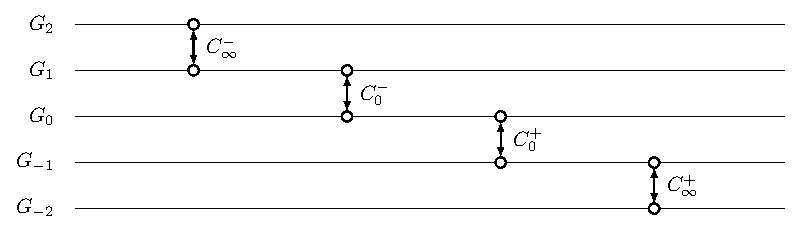
\includegraphics[scale=0.85]{figures/MixedG.png}
    \caption{Analytic structure of $G_{(2)}^Y(z)$ in the 3-state Potts model.}
    \label{fig:mixedG}
\end{figure}
%
Using their result one can infer the analytic structure of $G_{(2)}^Y(z)$, which is given in
Fig.\ref{fig:mixedG}. Therefore, using \eqref{2MMsaddle2} and the branch structure of
$G_{(2)}^Y(z)$, we should be able to determine the form of $W_{(2)}(z)$.

Define $U(z) = \frac{t_3}{4}z^2 + \frac{t_2}{2}z$, and label the physical sheet `0', such that the
saddle-point equation becomes
%
\begin{equation}
    W_{(2)}(z)_0 + W_{(2)}\big(-z-\frac{2t_2}{t_3}\big)_0 + G_{(2)}^Y(z)_0 = U(z).
\end{equation}
%
Let $W_{(2)}(z)_0$ have a compact branch cut on the interval $C_0^+=[a,b]$ (and thus
$W_{(2)}\big(-z-\frac{2t_2}{t_3}\big)_0$ has a cut on
$C_0^-=[-b-\frac{2t_2}{t_3},-a-\frac{2t_2}{t_3}]$), and $G_{(2)}^Y(z)_{-1}$ have a cut on
$C_{\infty}^+=[c,+\infty)$, as demonstrated in Fig.\ref{fig:mixedG}. We take $a,b,c\in \mathbb{R}$
and $a< b < c$. We now study the branch structure by analytically continuing through the various
branch cuts sequentially, and matching discontinuities.
\begin{enumerate}[label=(\roman*)]
    \item First, analytically continuing through the physical cut $C_0^+$ takes $W_{(2)}(z)_0 \rightarrow
              W_{(2)}(z)_1$, and we get
          \begin{equation}
              W_{(2)}(z)_1 + G_{(2)}^Y(z)_{-1} + W_{(2)}\big(-z-\frac{2t_2}{t_3}\big)_0 = U(z),
          \end{equation}
          from which we can infer that $W_{(2)}(z)_1$ has a cut along $C_0^-,C_0^+$, and $C_\infty^+$.

    \item Analytically continuing through $C_{\infty}^+$, we find
          \begin{equation}
              W_{(2)}(z)_2 + G_{(2)}^Y(z)_{-2}+W_{(2)}\big(-z-\frac{2t_2}{t_3}\big)_0 = U(z),
          \end{equation}
          and consequently $W_{(2)}(z)_2$ has a cut along $C_0^-$ and $C_{\infty}^+$.

    \item Circling $C_0^-$,
          \begin{equation}
              W_{(2)}(z)_3 + G_{(2)}^Y(z)_{-2}+W_{(2)}\big(-z-\frac{2t_2}{t_3}\big)_{1}=U(z),
          \end{equation}
          and so now we have a cut along $C_{\infty}^-, C_0^-, C_0^+$, and $C_{\infty}^+$.

    \item Circling $C_{\infty}^+$,
          \begin{equation}
              W_{(2)}(z)_4 + G_{(2)}^Y(z)_{-1} + W_{(2)}\big(-z-\frac{2t_2}{t_3}\big)_1 = U(z),
          \end{equation}
          which implies that $W_{(2)}(z)_4$ has a cut along $C_{\infty}^-, C_0^-$, and $C_{\infty}^+$.

    \item If we circle $C_0^-$, $G_{(2)}^Y(z)_{-1}\rightarrow G_{(2)}^Y(z)_0$ and
          $W_{(2)}\big(-z-\frac{2t_2}{t_3}\big)_1\rightarrow W_{(2)}\big(-z-\frac{2t_2}{t_3}\big)_0$, which
          implies that we return to sheet $W_{(2)}(z)_1$, and that these two are connected along $C_0^-$.
          Meanwhile, if we circle $C_{\infty}^-$,
          \begin{equation}
              W_{(2)}(z)_5 + G_{(2)}^Y(z)_{-1} + W_{(2)}\big(-z-\frac{2t_2}{t_3}\big)_2 = U(z),
          \end{equation}
          from which we deduce that $W_{(2)}(z)_5$ has a cut along $C_{\infty}^-$ and $C_{\infty}^+$.

    \item Circling $C_{\infty}^+$,
          \begin{equation}
              W_{(2)}(z)_6 + G_{(2)}^Y(z)_{-2}+W_{(2)}\big(-z-\frac{2t_2}{t_3}\big)_2=U(z),
          \end{equation}
          from which we infer that $W_{(2)}(z)_6$ has branch cuts along $C_{\infty}^-, C_0^+$, and
          $C_{\infty}^+$.

    \item At this point, if we circle $C_{\infty}^-$, $G_{(2)}^Y(z)_{-2}$ remains unchanged and
          $W_{(2)}\big(-z-\frac{2t_2}{t_3}\big)_2\rightarrow W_{(2)}\big(-z-\frac{2t_2}{t_3}\big)_1$, which
          tells us that $W_{(2)}(z)_6\rightarrow W_{(2)}(z)_3$. However, if we circle $C_0^+$, we find
          \begin{equation}
              W_{(2)}(z)_7 + G_{(2)}^Y(z)_{-2} + W_{(2)}\big(-z-\frac{2t_2}{t_3}\big)_3 = U(z),
          \end{equation}
          and so $W_{(2)}(z)_7$ has cuts along $C_{\infty}^-, C_0^-, C_0^+$.

    \item Circling $C_{\infty}^-$ gives
          \begin{equation}
              W_{(2)}(z)_8 + G_{(2)}^Y(z)_{-2} + W_{(2)}\big(-z-\frac{2t_2}{t_3}\big)_4 = U(z),
          \end{equation}
          and so $W_{(2)}(z)_8$ has cuts along $C_{\infty}^-$, and $C_0^+$. If we circle the latter, we find
          $W_{(2)}\big(-z-\frac{2t_2}{t_3}\big)_4\rightarrow W_{(2)}\big(-z-\frac{2t_2}{t_3}\big)_1$ and
          $G_{(2)}^Y(z)_{-2}$ remains unchanged, implying $W_{(2)}(z)_8 \rightarrow W_{(2)}(z)_3$.

    \item Finally, if we circle $C_0^-$ of $W_{(2)}(z)_7$
          \begin{equation}
              W_{(2)}(z)_9 + G_{(2)}^Y(z)_{-2}+W_{(2)}\big(-z-\frac{2t_2}{t_3}\big)_8 = U(z),
          \end{equation}
          which implies $W_{(2)}(z)_9$ has a single cut along $C_0^-$, terminating the sheet structure.
\end{enumerate}
%
\begin{figure}
    \centering
    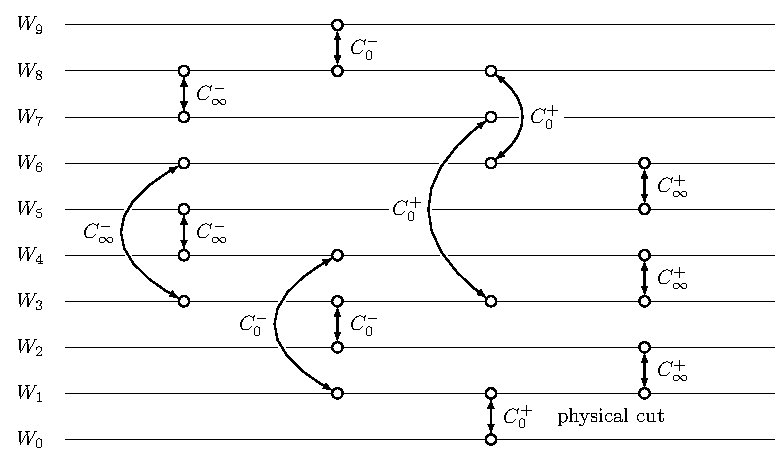
\includegraphics[scale=0.85]{figures/MixedW.png}
    \caption{Analytic structure of $W_{(2)}(z)$ in the 3-state Potts model.}
    \label{fig:Wstruct}
\end{figure}
%
The entire analytic structure is depicted in Fig.\ref{fig:Wstruct}.

We therefore find that the branch structure predicted by the loop equation solution is in agreement
with the solution found in \cite{Niedner:2016skw}. Moreover, one may explicitly compare the
asymptotics of the resolvent on each sheet, given in Appendix B, and see that it is in accord with
the saddle-point solution on each sheet, using the asymptotics of $G_{(2)}^Y(z)$ given in
\cite{Niedner:2016skw}.

\subsection{Free boundary conditions}

Let us choose a basis for the potential \eqref{3PottsFixed} given by $M_1 = X_1 + X_2 + X_3, M_2 =
    X_1 - X_2 + X_3, M_3 = X_1 + X_2 - X_3$. Then computing the resolvent corresponding to the free
boundary condition, $W_{(3)}(z)$, is equivalent to computing the planar resolvent of the matrix
$M_1$ with the following potential,
%
\begin{multline}
    \label{freeAction}
    V(M_1,M_2,M_3) =  \text{Tr} \bigg( \frac{(t_2-2)}{4}M_1^2 + \frac{t_2}{4}(M_2^2 + M_3^2 - M_1 M_2 + M_2 M_3 \\
    - M_3 M_1) + \frac{t_3}{8}(M_2^2 M_1 + M_3^2 M_1 + M_2^2 M_3 \\
    + M_3^2 M_2  - M_1^2 M_2 - M_1^2 M_3) + \frac{t_3}{12} M_1^3\bigg).
\end{multline}
%
As in the case of the mixed boundary condition, one must extend to level 6 to find a complete set
of constraints.

The model, as written, possesses a $\mathbb{Z}_2$ symmetry relating $M_2$ and $M_3$. However, the
correlators also possesses a further set of constraints, owing to their origin in the 3-state Potts
model, that are not manifest in \eqref{freeAction}. These are given by
%
\begin{equation}
    \label{extraCon}
    W_{2}(z) = \frac{1}{3} \Delta W_{(3)} (z),
\end{equation}
%
which is easily deduced by rewriting the terms in the original basis and imposing the full $S_3$
symmetry in the expectation value.

Applying the elimination procedure and \eqref{extraCon}, one can determine the spectral curve for
the free spin resolvent, given by an algebraic equation that is degree 5 in $z$ and degree 5 in the
resolvent $W_{(3)}(z)$. Furthermore, with the relation
%
\begin{equation}
    \label{strange}
    G_{(3)}^Y(z) = z + W_{(3)}(z),
\end{equation}
%
one recovers the spectral curve for $G_{(3)}^Y(z)$ of Atkin et al. The analytic structure of
$W_{(3)}(z)$ is provided in Fig.\ref{fig:FreeW}.

\begin{figure}
    \centering
    \includegraphics[scale=0.85]{figures/FreeW.png}
    \caption{Analytic structure of $W_{(3)}(z)$ in the 3-state Potts model.}
    \label{fig:FreeW}
\end{figure}

\subsection{An `odd' boundary condition}

Returning to \eqref{freeAction}, it is also possible to use the loop equation approach to calculate
the planar resolvent of $M_2$. We shall call this the `odd' boundary condition and label the
resolvent $W'(z)$. As with the free spin resolvent, there is a supplementary constraint on the
resolvent functions that is not manifest in the potential,
%
\begin{equation}
    \label{wextraCon}
    W'_1(z) = 2 W'_3(z) + \Delta' W'(z),
\end{equation}
%
where the $\Delta'$ is understood to correspond to insertions of the matrix $M_2$. Once again, we
find $n_{\text{max}} = 6$, and the resulting spectral curve is degree 14 in $W'(z)$ and degree 13
in $z$.

At the moment, it is unclear what the physical interpretation of this object might be. It may be
related to the $W_{X_1 - X_2}(z)$ one-loop function of the Ising model coupled to 2D gravity
\cite{Atkin:2010yv}, but further study of the scaling limit would be needed to demonstrate this.

\subsection{$U$ boundary conditions}

To study the $U = X_1 + \omega X_2 + \omega^2 X_3$ boundary condition we choose the basis $U,
    U^\dagger$ and $X=X_1 +X_2 + X_3$. The potential is equivalent to the action \eqref{dual} up to a
scaling of the matrices,
%
\begin{multline}
    V(X,U,U^\dagger) =  \text{Tr}\bigg( \frac{(t_2 - 3)}{6}X^2 + \frac{t_2}{3}UU^\dagger + \frac{t_3}{9}(UU^\dagger X + X U^\dagger U) \\
    + \frac{t_3}{27} (X^3 + U^3 + (U^\dagger)^3)\bigg).
\end{multline}
%

The structure of the loop equations is quite simple, and one may expect $n_{\text{max}}=5$, as in
the case of the fixed boundary condition. However, unlike the previous cases, applying the
algorithm to compute the resolvent of $U$ does not result in a closed system of equations, even if
we consider loop equations of level 6. Instead, we obtain a polynomial equation relating the
resolvent and the level 1 loop function $W_{X}(z)$.

We have extended this to level 7 and found that the system of equations still does not close. With
the relative simplicity of the potential, this strongly suggests that this resolvent cannot be
determined using our loop equation approach.

\section{Dilute Ising Model}

We now turn our attention to the dilute Ising model on random planar graphs, given by the following
matrix integral,
%
\begin{equation}
    \label{diluteQ}
    Z = \int [dY] \prod_{i=1}^q [dX_i] e^{-N\text{Tr}\left( \frac{1}{2}Y^2 + \frac{t_0}{3} Y^3 + \sum_{i=1}^q \left(\frac{t_2}{2} X_i^2 + \frac{t_3}{3} X_i^3 - Y X_i\right) \right)},
\end{equation}
%
for $q=2$. For arbitrary $q$, this matrix integral represents the dilute $q$-state Potts model,
first studied by Zinn-Justin \cite{ZinnJustin:1999jg} using the saddle-point method. The parameter
$t_0$ determines the dilution of random graphs, i.e. the number of sites not occupied by the spins
$\{X_i\}_{i=1}^q$. For $t_0=0$ the integral over $Y$ may be evaluated, and one recovers the
$q$-state Potts model \eqref{eq1}. The resolvent corresponding to $p=1$ fixed spin boundary
conditions was computed for $q=1,2$, and $3$, by means of computing the auxiliary $G$-function
\eqref{eq7} corresponding to $Y$-boundary conditions. We will reproduce these results using the
loop equation formalism.

In this section, we will discuss the vacant, fixed, and free boundary conditions in the dilute
Ising model. As noted in Chapter 2, these boundary conditions represent three out of the four fixed
lattice realisations of the physical conformally invariant boundary states. We have not determined
the remaining `partially fixed' boundary condition, which we expect to be captured by the planar
resolvent
%
\begin{equation}
    W_{p.f.}(z) = \frac{1}{N} \left\langle \text{Tr}\, \frac{1}{z-(X_1 + Y)}\right\rangle.
\end{equation}

\subsection{Vacant boundary conditions}

The boundary condition in which all the sites on the boundary are left vacant is realised by the
resolvent
%
\begin{equation}
    \label{vacantRes}
    W_Y(z) = \frac{1}{N} \left\langle \text{Tr} \, \frac{1}{z-Y} \right\rangle.
\end{equation}
%
This may be determined using the loop equation approach with $n_{\text{max}}=5$, resulting in a
spectral curve that is degree 6 in $z$ and degree $4$ in $W_Y(z)$. The analytic structure is
presented in Fig.\ref{fig:VacIsing}.

\begin{figure}
    \centering
    \includegraphics[scale=0.85]{figures/VacIsing.png}
    \caption{Analytic structure of $W_{Y}(z)$ in the dilute Ising model.}
    \label{fig:VacIsing}
\end{figure}

\subsection{Fixed boundary conditions}

The fixed spin boundary condition, $W_{(1)}(z)$, may be computed using loop equations with
$n_{\text{max}}=5$, resulting in a spectral curve that is degree 8 in $z$ and degree 5 in
$W_{(1)}(z)$. The analytic structure is presented in Fig.\ref{fig:DIsing}.

\begin{figure}
    \centering
    \includegraphics[scale=0.85]{figures/DFixedIsing.png}
    \caption{Analytic structure of $W_{(1)}(z)$ in the dilute Ising model.}
    \label{fig:DIsing}
\end{figure}

We note that when dilution is turned off we recover the spectral curve \eqref{IsingSpec}, as
expected. The introduction of vacancies fundamentally alters the analytic structure of the Ising
spectral curve from a curve that is degree 3 in the resolvent to a degree 5 curve, and this allows
one to generate even higher order critical behaviour. It was argued in \cite{ZinnJustin:1999jg}
that this extra structure admits a new critical point with $\gamma_s=-\frac{1}{4}$, which
corresponds to the universality class of the $c=7/10$ tricritical Ising model coupled to 2D
gravity.

\subsection{Free boundary conditions}

To study the free boundary condition we choose the basis $M_1 = X_1 + X_2, M_2=X_1 - X_2$, and
calculate the planar resolvent of $M_1$. The potential is given by
%
\begin{multline}
    \label{freeDiluteIsing}
    V(Y,M_1,M_2) = N\text{Tr}\bigg( \frac{1}{2} Y^2 + \frac{t_0}{3}Y^3 + \frac{t_2}{4}(M_1^2 + M_2^2 ) \\
    + \frac{t_3}{12}(M_1^3 + 3M_1 M_2^2) - YM_1 \bigg).
\end{multline}
%
Extending to level $n_{\text{max}}=6$ we obtain a closed system of loop equations from which we can
compute the spectral curve. The final result is degree 10 in $z$ and degree 10 in $W_{(2)}(z)$. The
analytic structure is identical to the mixed boundary condition in the 3-state Potts model,
Fig.\ref{fig:Wstruct}.

\section{Dilute Potts Model}

Finally, we consider the dilute Potts model on random planar graphs, given by \eqref{diluteQ} for
$q=3$. In this section, we will discuss the vacant and fixed spin boundary conditions, which we
have calculated using the loop equation approach.

\subsection{Vacant boundary conditions}

The vacant boundary condition $W_Y(z)$ may be calculated by extending to variations of level
$n_{\text{max}}=7$. The spectral curve is degree 10 in the boundary cosmological constant $z$, and
degree 6 in the resolvent $W_Y(z)$. The analytic structure is presented in Fig.\ref{fig:VacPotts}.

\begin{figure}
    \centering
    \includegraphics[scale=0.85]{figures/VacPotts.png}
    \caption{Analytic structure of $W_{Y}(z)$ in the dilute Potts model.}
    \label{fig:VacPotts}
\end{figure}

\subsection{Fixed boundary conditions}

The fixed boundary condition, $W_{(1)}(z)$, may also be calculated with $n_{\text{max}}=7$. In this
case, the spectral curve is degree 16 in the boundary cosmological constant $z$ and degree 9 in the
resolvent $W_{(1)}(z)$. The analytic structure is presented in Fig.\ref{fig:DPotts}.

As with the dilute Ising model, one recovers the spectral curve of the critical Potts model when
the dilution is turned off. In \cite{ZinnJustin:1999jg} it was argued that the extra structure
generated by introducing dilution allows for a new critical point with $\gamma_s = -\frac{1}{6}$,
which corresponds to the universality class of the $c=6/7$ tricritical Potts model.

\begin{figure}
    \centering
    \includegraphics[scale=0.85]{figures/DFixedPotts.png}
    \caption{Analytic structure of $W_{(1)}(z)$ in the dilute Potts model.}
    \label{fig:DPotts}
\end{figure}

\section{Discussion}

In this chapter, we developed an algorithm for systematically computing and solving the loop
equations of general multi-matrix models, in the goal of finding the spectral curve for the planar
resolvent of a given matrix degree of freedom. We then focused our attention on the 3-state Potts
model, where we successfully computed the planar resolvents describing fixed, mixed, and free
boundary conditions using this technique. While the fixed and free boundary conditions were
manifestly in agreement with the literature, more care was required for the mixed boundary
condition. Through studying the analytic structure predicted by the saddle-point solution, we were
able to show that this too was consistent with the results of Atkin et al. We then considered some
non-standard resolvents, including a new `odd' boundary condition, which was susceptible to the
loop equation strategy, and a $U$ boundary condition which we were not able to solve. Following
this, we discussed the dilute Ising and Potts models, where we computed the resolvents
corresponding to various boundary conditions, in agreement with the results of Zinn-Justin.

There are many ways to continue this work. Our procedure is algorithmic in nature and so it would
be interesting to apply this to a wide variety of models for which the planar resolvent is known or
unknown. In the context of three-matrix models more generally, it would be interesting to
understand the criteria under which a resolvent is calculable. As we have seen from our results, we
were able to calculate the planar resolvent for particular systems with full $S_3$ symmetry under
interchange of the matrix degrees of freedom \eqref{mixedAction}, and for systems where there is a
residual $\mathbb{Z}_2$ symmetry under the remaining degrees of freedom, with an auxiliary
condition reducing the number of level-1 resolvent functions \eqref{freeAction}. Determining
whether this can be elevated to a general principle governing solvability of correlators in the
three-matrix model would be an exciting challenge. One immediate offshoot of this would be the
calculation of planar resolvents describing boundary conditions that interpolate between the fixed,
mixed and free boundary states analogous to \cite{Carroll:1997tr,Atkin:2012fx}. This would allow us
to directly study the boundary renormalisation group flow relating the different boundary states,
which is expected to induce a partial ordering of the spectrum of boundary states, conforming with
the boundary analogue of the $c$-theorem \cite{Zamolodchikov:1986gt}, which was first conjectured
in \cite{Affleck:1991tk}, and subsequently proven by Friedan and Konechny \cite{Friedan:2003yc}.

Another interesting avenue of research would be to investigate whether we could generalise the
algorithm developed in this chapter for a wider variety of correlators and matrix models, such as
the $q$-state Potts model where $q$ is taken to be non-integer. This is possible for the simple
example of the fixed-spin boundary condition \cite{Bonnet:1999nf}. Whether we could do the same for
general boundary conditions and reproduce the saddle-point results of Chapter 3 is an open
question. This would provide further insight into the nature of the allowed $G$-functions and
corresponding boundary conditions in the $q$-state Potts model. It would also be useful for
studying the expression for the New boundary condition determined in Chapter 4, which is given by a
non-standard resolvent function that would not immediately be amenable to calculation through the
loop equation method devised in this chapter.

Finally, it would be fruitful to extend our work to the calculation of observables in multi-matrix
models beyond the planar limit. It is well known that the planar resolvent forms the initial data
for higher-genus and multi-boundary correlators in the one- and two-matrix models
\cite{Eynard:2002kg,Eynard:2004mh,Eynard:2008we}, and that this may be extended to certain
multi-matrix models \cite{Borot:2009ia}. It would be interesting to see whether one could reframe
the method of loop equations for various boundary conditions in the 3-state Potts model such that
one can calculate higher-order correlation functions in an analogous topological recursion
procedure. This would allow, for example, the computation of cylinder amplitudes for different
boundary states, and might provide valuable information as to how to interpret the results of
Chapter 3.